\documentclass{report}
\usepackage[utf8]{inputenc}
\usepackage{amsthm}
\usepackage{amsmath, mathtools, amsfonts,amssymb}
\usepackage{graphicx}
\usepackage{verbatim}
\usepackage{fancyhdr}
\usepackage{subfigure}
\usepackage{float}
% Code
\usepackage{listings} 
\usepackage{algorithm}
\usepackage{algpseudocode}
% Margins
\usepackage{geometry}
%\geometry{margin=1in} %% 

% Graphics
\usepackage{tikz}
\usetikzlibrary{matrix} % matrices
\usepackage{tikz-qtree} % Simple trees

% Theorems/etc.
\newtheorem{pic}{Figure}
\numberwithin{pic}{section}
\newtheorem{lem}{Lemma}
\numberwithin{lem}{section}
\newtheorem{thm}{Theorem}
\numberwithin{thm}{section}
\newtheorem{cor}{Corollary}
\numberwithin{cor}{section}

\theoremstyle{definition}
\newtheorem{ex}{Example}
\numberwithin{ex}{section}
\newtheorem{defn}{Definition}
\numberwithin{defn}{section}
\theoremstyle{definition}
\newtheorem{prob}{Problem}

\theoremstyle{remark}
\newtheorem*{con}{Conjecture}
\newtheorem{rem}{Remark}
\newtheorem*{cex}{Counterexample}
\newtheorem*{ts}{T.S.}

%%% COMMANDS %%%
% Sets
\newcommand{\set}[1]{\ensuremath{\left\{ #1\right\}}} % write sets
\newcommand{\e}{\ensuremath{\epsilon}} % Epsilon
\newcommand{\R}{\ensuremath{\mathbb{R}}} % Real Numbers
\newcommand{\N}{\ensuremath{\mathbb{N}}} % Natural numbers
\newcommand{\Q}{\ensuremath{\mathbb{Q}}} % Rationals
\newcommand{\I}{\ensuremath{\mathbb{I}}} % Irrational Numbers
\newcommand{\Z}{\ensuremath{\mathbb{Z}}} % Integers
% Easier Delimiters?
\newcommand{\lr}[2]{\ensuremath{\left#1 #2 \right #1}}
% Absolute Value
\newcommand{\abs}[1]{\ensuremath{\left| #1 \right|}}
% Landau Notation
\newcommand{\Oh}{\ensuremath{\mathcal{O}}} %%% IN MATH MODE
\newcommand{\oh}{\ensuremath{\mathcal{o}}} %%% IN MATH MODE
% Display style fractions
\newcommand{\Frac}[2]{\displaystyle \frac{#1}{#2}}
% Display style limits
\newcommand{\Lim}[2]{\displaystyle \lim_{#1}{#2}}

%%% Preference Stuff %%%
\setcounter{section}{-1}
\renewcommand\qedsymbol{{$\blacksquare$}}
% Enumerate
\renewcommand{\labelenumi}{(\alph{enumi})}
\renewcommand{\labelenumii}{\roman{enumii}}
% change proof environment
\renewcommand*{\proofname}{Pf}
% Line Spacing
\renewcommand{\baselinestretch}{1.5}
% Indentation
\newlength\tindent
\setlength{\tindent}{\parindent}
\setlength{\parindent}{0pt}
\renewcommand{\indent}{\hspace*{\tindent}}


% Set title
\title{Computational Math Project\\
  {\large Illinois Institute of Technology}
}
\author{
  Miles Bakenhus 
  \and
  Ahmed Lodhika 
  \and
  Gunjan Sharma 
  \and
  Quinn Stratton 
  \and
  Jan-Eric Sulzbach 
}
\date{\today}
\begin{document}


\fancyhead[l]{}
\fancyhead[c]{}
\fancyhead[r]{}
% \pagestyle{fancy}

\maketitle

\tableofcontents


\section{Introduction}

\section{Theory}
\begin{thm}
If $A$ is a tridiagonal matrix. Then R in the the product $A=QR$ is a upper triangular matrix with non zero entries only in the diagonal and the two super diagonals.
\end{thm}
\[A=\begin{pmatrix}
a_{11} & a_{12} &  &   \\ 
a_{21} & a_{22} & a_{23} &    \\ 
 & \ddots & \ddots & \ddots   \\ 
   &  & a_{m m-1} & a_{mm}
\end{pmatrix}~,~R=\begin{pmatrix}
r_{11} & r_{12} & r_{13} &  \\ 
 & \ddots & \ddots & \ddots \\ 
 &  & \ddots & \ddots \\ 
 &  &  & r_{mm}
\end{pmatrix}  \]
\begin{proof}
To prove the statement we will use the classical Gram-Schmidt method for the QR decomposition.\\
Step 1: we want to show that $q_j$ has the form $q_j=\begin{pmatrix}
* \\ 
\vdots \\ 
* \\ 
0 \\ 
\vdots
\end{pmatrix} \leftarrow j+1\text{-th entry}$.\\
We prove this by induction:
\begin{description}
\item[Base step] $j=1$ the if we assume that $\|a_1\|=1$ then $q_1=a_1$ thus
\[q_1= \begin{pmatrix}
a_{11} \\ 
a_{21} \\ 
0 \\  
\vdots
\end{pmatrix}\]
\item[Induction step] Assume that the statement holds for $j-1$. Then
\[v_j=a_j-\sum_{k=1}^{j-1} (q_k^* a_j)q_k~\text{ and } q_j= v_j/\|v\|_j\]
and by using the form of $q_{j-1}$ we obtain
\[q_j= \begin{pmatrix}
0\\ 
\vdots \\ 
a_{j-1, j} \\ 
a_{jj} \\ 
a_{j+1,j} \\
0\\
\vdots
\end{pmatrix}-\sum_{k=1}^{j-1} \begin{pmatrix}
*\\ 
\vdots \\ 
\vdots \\ 
* \\ 
0 \\
\vdots\\
\vdots
\end{pmatrix}\leftarrow k+1\text{-th entry}= \begin{pmatrix}
*\\ 
\vdots \\ 
\vdots \\ 
* \\ 
0 \\
\vdots\\
\vdots
\end{pmatrix}\leftarrow j+1\text{-th entry} \]
\end{description}
Step 2: Compute $r_{ij}$ in the CGS method\\
For $j=1$ to $n$ and for $i=1$ to $j-1$: $r_{ij}= q_i^*a_j$.
Then by step 1 we obtain that $r_{ij}=0$ if $i\leq j-3$ since then by the form of the vectors $q_{j-3}$ and $a_j$
\[0=\begin{pmatrix}
* \\ 
\vdots  \\ 
* \\ 
0 \\ 
0 \\
0\\
0 \\
\vdots \\ 
0
\end{pmatrix}^*\begin{pmatrix}
0 \\ 
\vdots  \\ 
0 \\ 
* \\ 
* \\ 
*\\
0\\
\vdots\\
0
\end{pmatrix} \leftarrow j\text{-th enttry} \]
The above argument holds for all $i\leq j-3$. 
\end{proof}
Now we want to generalize the above ideas to the case where A still has only three non-zero bands.
But now, the lower band has the distance $k-1$ from the diagonal and the upper band has the distance $l-1$ from the diagonal.\\
Consider the following example for A: 
\begin{figure}[	H]
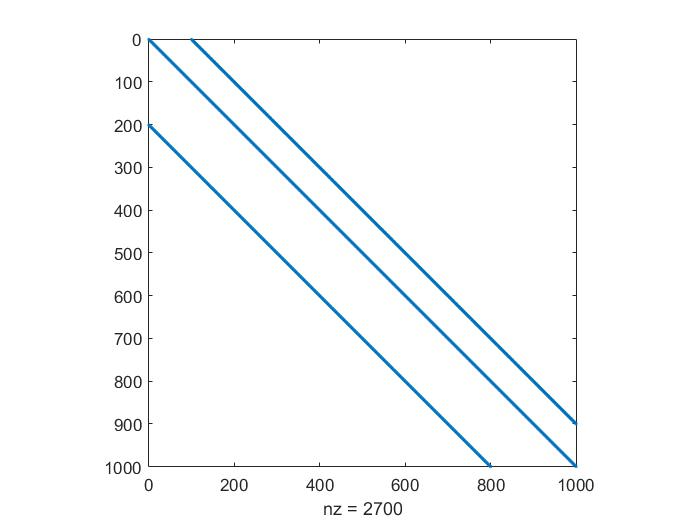
\includegraphics[scale=0.3]{example1.jpg}
\caption{$k=200$ and $l=100$}
\end{figure}

\begin{thm}[General case]
The upper triangular matrix $R$ in the $QR$ decomposition of $A$ has a $k+l$-band structure.
\end{thm}
\begin{proof}
From the classical Gram Schmidt method we immediately see, that in the worst case, the first $j+k$ entries are non zero.
Therefore, the inner product in the computation of the entries $r_{ij}$ is only zero if $i<j-l-k+2$. 
\end{proof}
Example of a matrix close to the worst case, where the number of non-zero entries (nz) increases by order 50:
\begin{figure}[H] 
    \subfigure[A]{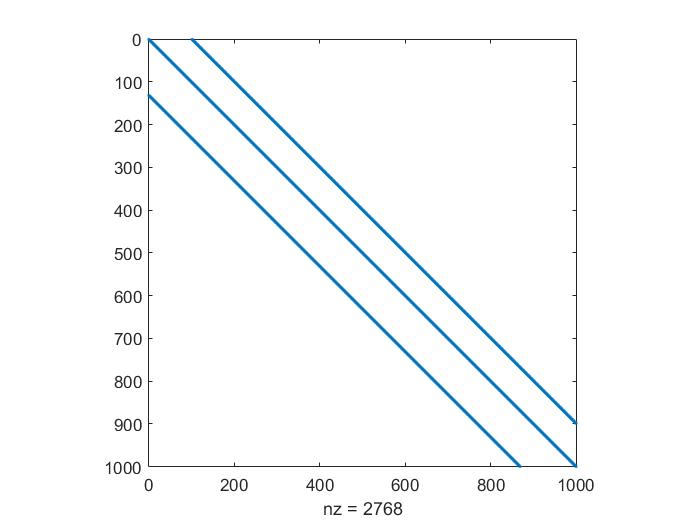
\includegraphics[width=0.49\textwidth]{example2.jpg}} 
    \subfigure[R]{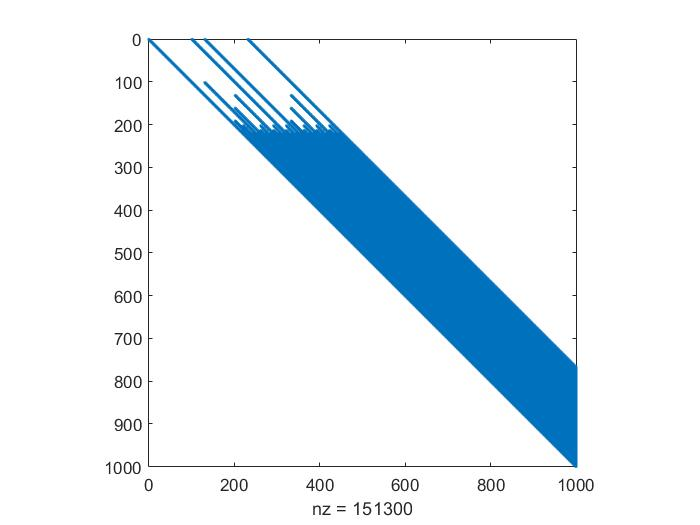
\includegraphics[width=0.49\textwidth]{example3.jpg}}  

    \caption{$k=131$ and $l=101$}
\end{figure} 
A special case occurs when $k=l$. Then again $R$ has only three non-zero band, i.e the diagonal, the band on the upper diagonal that has a distance $k$ to the diagonal and the upper diagonal that has a distance $2k$ to the diagonal.\\
Again we have an example for this case:
\begin{figure}[H] 
    \subfigure[A]{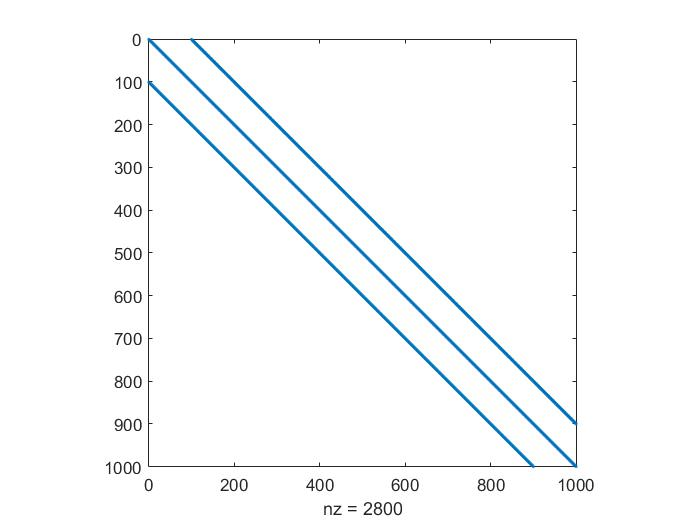
\includegraphics[width=0.49\textwidth]{example4.jpg}} 
    \subfigure[R]{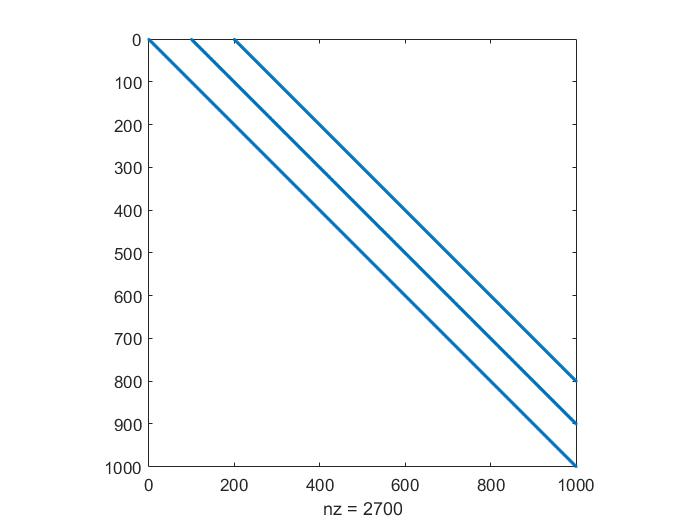
\includegraphics[width=0.49\textwidth]{example5.jpg}}  

    \caption{$k=l=100$ }
\end{figure} 
\end{document}